El presente proyecto adopta un enfoque metodológico mixto, que combina elementos cuantitativos y cualitativos para abordar de manera completa la pregunta de investigación. La dimensión cuantitativa se basa en el análisis de características acústicas de señales vocales, el entrenamiento y evaluación de modelos de machine learning y la medición objetiva del desempeño del sistema mediante métricas computacionales. Ahora, la dimensión cualitativa se sustenta en la evaluación perceptual de las propuestas generadas por el sistema a través de pruebas de escucha con usuarios de distintos niveles de experiencia. Este enfoque mixto resulta el más adecuado para la pregunta de investigación porque, como señalan Vanka et al. en [1], la mezcla de audio es un proceso que involucra tanto decisiones técnicas medibles como criterios estéticos y creativos que solo pueden ser evaluados subjetivamente. Un enfoque exclusivamente cuantitativo no capturaría la naturaleza creativa del proceso, mientras que uno solamente cualitativo no permitiría verificar el funcionamiento técnico del sistema propuesto [1].

El diseño del estudio es de tipo descriptivo-exploratorio con un componente de desarrollo tecnológico. Es descriptivo porque se busca caracterizar las propiedades acústicas de señales vocales presentes en grabaciones profesionales e identificar los patrones de procesamiento más comunes en cadenas de mezcla vocal. Es exploratorio porque el desarrollo de sistemas inteligentes especializados en mezcla vocal sigue siendo un campo poco explorado. Martínez Ramírez y Reiss en [5], identificaron que la voz es significativamente más difícil de modelar que otros instrumentos debido a su complejidad tímbrica y variabilidad estilística, lo que justifica un abordaje exploratorio hacia nuevas aproximaciones para este contexto específico [5]. El aspecto de desarrollo tecnológico se apoya con el diseño descriptivo: los hallazgos del análisis acústico, la revisión de patrones de procesamiento y la evaluación con usuarios alimentan directamente el diseño e implementación del sistema inteligente propuesto.

Además, el proyecto se apoya en una perspectiva de sistemas inteligentes asistivos y contextuales. Esto significa que la plataforma no se crea como un sistema de caja negra orientado a reemplazar completamente el criterio del ingeniero, sino como una herramienta capaz de generar propuestas iniciales de procesamiento que puedan ser ajustadas por el usuario. Esta decisión metodológica se sustenta en los planteamientos de Lefford et al. en [8], quienes afirman que las decisiones de mezcla no dependen únicamente de reglas técnicas, sino también del contexto musical, el género, la intención estética, las expectativas del usuario y las condiciones específicas de cada producción. Por esta razón, el sistema propuesto deberá considerar no sólo las características acústicas de la señal vocal, sino también información contextual básica como el género musical, el tipo de voz, la intención sonora buscada y cuando sea posible, una referencia musical proporcionada por el usuario [8].

En cuanto a los datos y fuentes, el proyecto requiere tres tipos de datos principales. El primero corresponde a grabaciones vocales crudas (sin procesar) y sus versiones procesadas con cadenas de mezcla aplicadas por ingenieros profesionales. Este tipo de datos de pares crudos/procesados constituye la base de entrenamiento de los sistemas de aprendizaje profundo para mezcla automática, tal como fue utilizado por Martínez Ramírez y Reiss en [5], quienes emplearon el dataset Open Multitrack Testbed junto con MedleyDB para entrenar autoencoders a partir de stems crudos y procesados. El segundo tipo corresponde a datos de evaluación perceptual, recolectados mediante pruebas de escucha con usuarios y el tercer tipo corresponde a datos semánticos y contextuales relacionados con la manera en que los usuarios describen objetivos sonoros, por ejemplo términos como "brillante", "cálido", "opaco", "presente", "saturado" o "agresivo". Este tercer componente se justifica gracias al trabajo de Venkatesh, Moffat y Miranda en [9], quienes demostraron que los word embeddings pueden utilizarse para traducir descriptores semánticos a configuraciones de ecualización, permitiendo que usuarios sin formación técnica comuniquen sus objetivos creativos de manera más intuitiva [9].

\begin{figure}[h!]
\centering
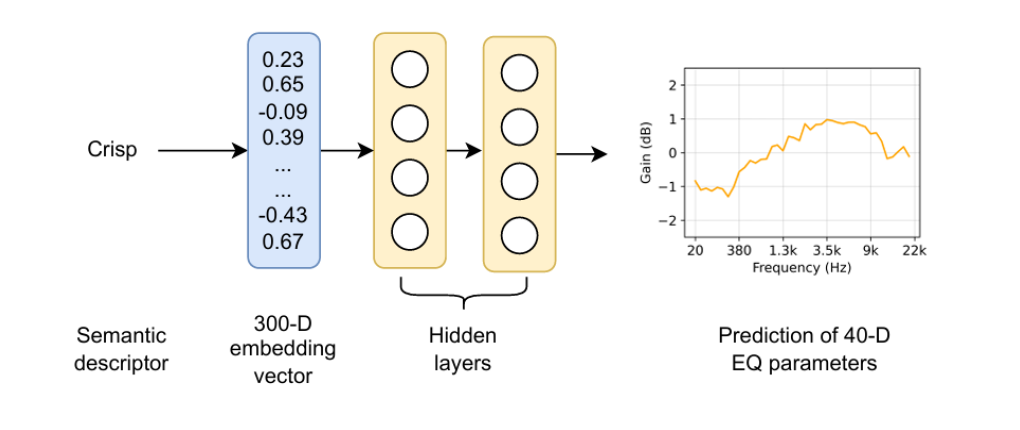
\includegraphics[width=0.7\textwidth]{images/fig8.png} 
\caption{Esquema de traducción de descriptores semánticos a parámetros de ecualización mediante word embeddings. Fuente: Venkatesh, Moffat y Miranda [9].}
\label{fig:fig8}
\end{figure}

Las fuentes de datos primarias serán datasets académicos y de canciones ya publicadas y validados, entre los que destacan MedleyDB que contiene grabaciones multipista reales de canciones completas en múltiples géneros con stems separados. Para el componente vocal, se priorizarán grabaciones vocales crudas y procesadas provenientes de datasets abiertos, repositorios multipista y, si es necesario, muestras propias grabadas bajo condiciones controladas. Para el componente semántico, se tomará como referencia el dataset SocialEQ utilizado en [9], ya que permite relacionar descriptores subjetivos con curvas de ecualización. Finalmente, para la definición de métricas objetivas de análisis de mezcla, se tomarán como referencia los criterios utilizados por Mourgela et al. en [10], quienes analizaron una base de datos de más de 218.000 entradas de mezclas y masters a partir de variables como loudness integrado, true peak, clipping, compatibilidad mono, problemas de fase, compresión, amplitud estéreo y perfil tonal [10].

\begin{table}[h!]
\centering
\caption{Métodos de análisis de características de audio utilizados para evaluar aspectos técnicos de mezclas y masters. Fuente: Mourgela et al. [10]}
\label{tab:mourgela}
\begin{tabular}{|p{3.2cm}|p{9.5cm}|}
\hline
\textbf{Feature} & \textbf{Analysis Method} \\
\hline
Bit depth, sample rate & Extracted from file \\
\hline
Integrated loudness & Calculated based on the ITU BS.1770 standard [11] \\
\hline
True peak & Calculated based on the ITU BS.1770 standard [11] \\
\hline
Compression & Calculated based on dynamic ranges in decibels (dB) of a signal by measuring 20 times the base-10 logarithm of the ratio between its maximum and mean amplitudes. Dynamic ranges are then compared to empirical average genre-specific levels found in the industry. \\
\hline
Stereo Width Balance & Calculated based on the inter-channel level difference. \\
\hline
Mono compatibility & Calculated by examining the correlation between the mid and side signals derived from the left and right stereo channels. \\
\hline
Tonal Profile & Calculated by dividing its frequency spectrum into defined bands (20-250, 250-2000, 2000-8000, 8000-20000) and comparing the energy within each band to thresholds relating to perceptual weighting. \\
\hline
Clipping & Calculated by counting how many samples exceed the digital full scale (0 dBFS) threshold, as well as evaluating the extent of clipping based on the number of clipped samples (over 10000 clipped samples signify major clipping) \\
\hline
Phase issues & Assesses the presence of phase issues between the left and right channels of a stereo audio signal by calculating the mean absolute phase difference and comparing it to a predefined threshold of 1.7 radians, set heuristically based on typical values observed in songs with noticeable out-of-phase issues. \\
\hline
\end{tabular}
\end{table}

Las herramientas y tecnologías que se emplearán en el desarrollo del proyecto se organizan en cuatro niveles. En el nivel de análisis acústico, se utilizará Python como lenguaje principal, junto con librerías especializadas como Librosa, Essentia, NumPy, SciPy y pyloudnorm para la extracción de características de audio. Entre estas características se contemplan la frecuencia fundamental, relación armónico-ruido (HNR), coeficientes mel-frequency cepstral (MFCC), centroide espectral, energía por bandas, rango dinámico, loudness integrado, true peak y medidas asociadas a estabilidad tonal y dinámica. Estos parámetros permiten construir una representación objetiva del perfil acústico de la voz y del comportamiento técnico de la mezcla.

En el nivel de modelado, se explorarán arquitecturas de machine learning y deep learning orientadas a la predicción de cadenas de procesamiento o parámetros de mezcla. Se tomarán como referencia los autoencoders profundos utilizados por Martínez Ramírez y Reiss en [5], las redes de convolución temporal y consolas diferenciables propuestas por Steinmetz et al. en [7], y los enfoques generativos como MEGAMI propuesto por Moliner et al. en [3]. Sin embargo, debido al alcance del presente anteproyecto, el objetivo no será replicar completamente estos sistemas, sino adaptar sus principios metodológicos al diseño de una plataforma especializada en mezcla vocal. En ese sentido, se priorizará un enfoque de estimación de parámetros y recomendación de cadenas, más que una transformación directa de audio completamente automática.

\begin{figure}[h!]
\centering
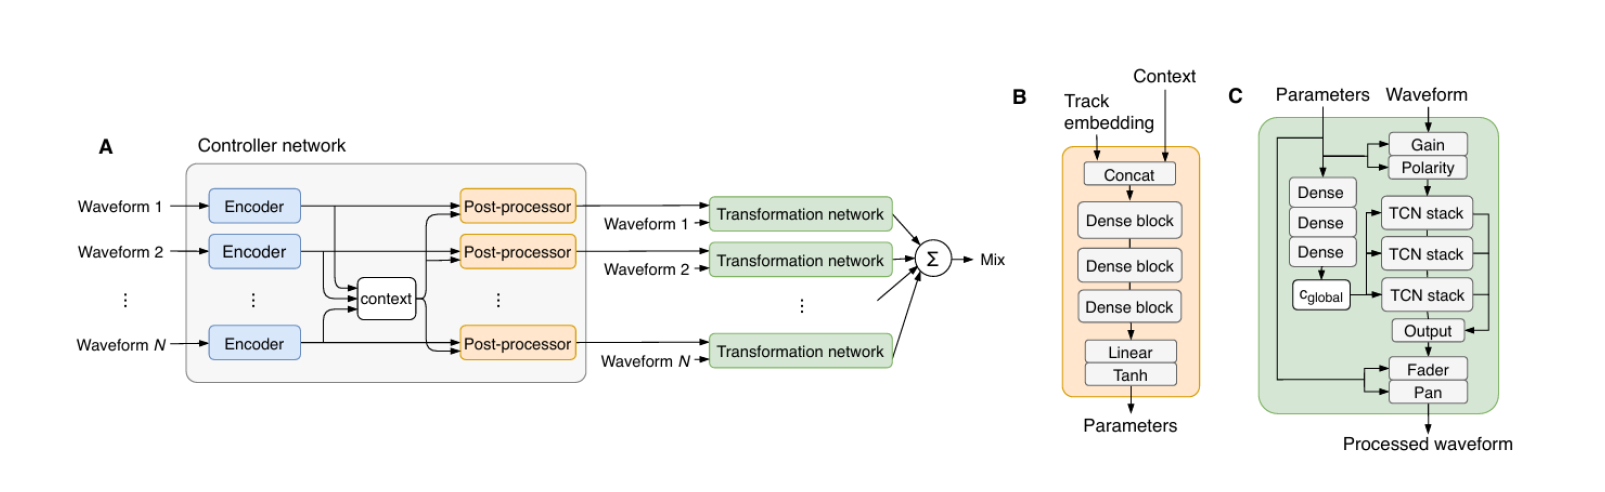
\includegraphics[width=0.9\textwidth]{images/fig10.png}
\caption{Diagrama de una consola de mezcla diferenciable orientada a la estimación de parámetros de procesamiento de audio. Fuente: Steinmetz et al. [7].}
\label{fig:fig10}
\end{figure}

En el nivel de interacción con el usuario, se considerará la posibilidad de integrar descriptores semánticos y referencias musicales como entradas complementarias del sistema. El uso de descriptores semánticos permitirá que el usuario indique una intención sonora de manera más natural, por ejemplo "quiero una voz más brillante" o "quiero una voz menos nasal", mientras que el uso de una canción de referencia permitirá orientar la propuesta hacia un estilo de mezcla específico. Este componente se relaciona con el trabajo de Diff-MST propuesto por Vanka et al. en [11], donde el sistema utiliza pistas crudas y una canción de referencia para estimar parámetros de una consola de mezcla diferenciable, conservando la posibilidad de realizar ajustes posteriores por parte del usuario [11]. Esta idea resulta especialmente pertinente para el presente proyecto, ya que permite mantener el control creativo del productor o ingeniero en lugar de sustituirlo por una decisión automática cerrada.

\begin{figure}[h!]
\centering
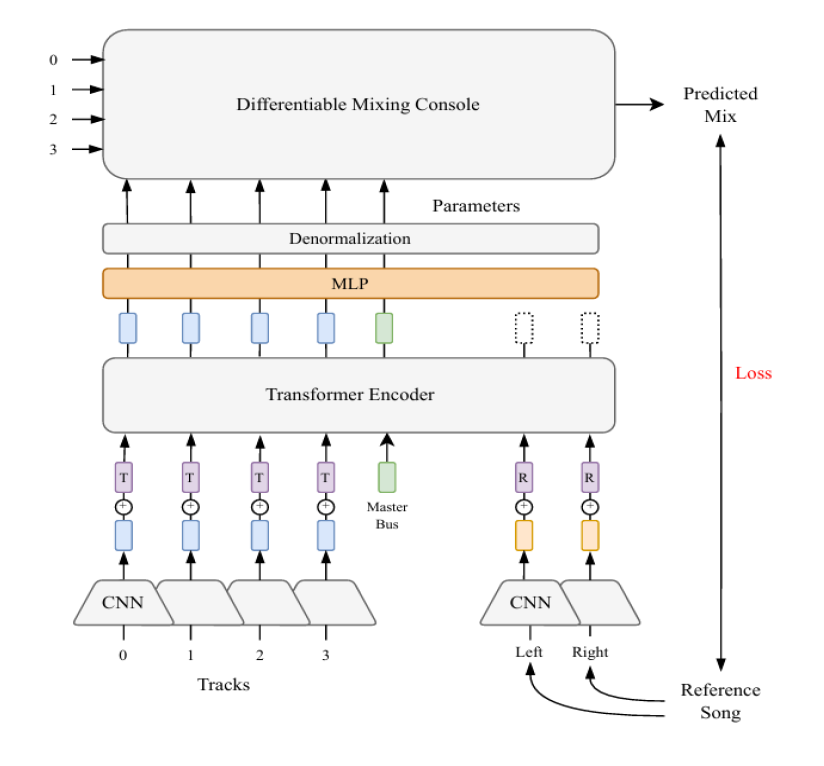
\includegraphics[width=0.9\textwidth]{images/fig11.png} 
\caption{Arquitectura de un sistema de transferencia de estilo de mezcla basado en pistas crudas, referencia sonora y estimación de parámetros mediante consola diferenciable. Fuente: Vanka et al. [11].}
\label{fig:fig11}
\end{figure}

En el nivel de evaluación se emplearán pruebas objetivas y subjetivas. Para la evaluación objetiva se calcularán métricas técnicas relacionadas con el comportamiento espectral, dinámico y espacial de las propuestas generadas por el sistema. Entre estas métricas se incluirán loudness integrado, true peak, detección de clipping, rango dinámico, balance tonal por bandas, estabilidad de la señal vocal, similitud espectral con la referencia y consistencia de los parámetros sugeridos. Estas métricas se seleccionan teniendo en cuenta los criterios utilizados por Mourgela et al. en [10], quienes evidenciaron que problemas como exceso de loudness, clipping, desbalance tonal, subcompresión, sobrecompresión y problemas de compatibilidad mono siguen siendo recurrentes en producciones realizadas por usuarios reales. Para la evaluación perceptual, se empleará el Web Audio Evaluation Tool o una plataforma equivalente de pruebas de escucha, siguiendo metodologías utilizadas en investigaciones previas sobre mezcla automática [2], [7].

El procedimiento de análisis se organiza en cinco fases consecutivas. La primera fase consiste en la revisión y ajuste del protocolo de revisión sistemática de literatura, con el fin de consolidar los artículos relacionados con mezcla automática, inteligencia artificial aplicada al audio, procesamiento vocal, sistemas inteligentes asistivos, descriptores semánticos y evaluación perceptual. En esta fase se clasifican los documentos según su nivel de relación con el proyecto y se determina cuáles aportan al marco conceptual, al marco referencial o al diseño metodológico.

La segunda fase corresponde a la adquisición y preparación de datos. En esta etapa se identificarán y seleccionarán datasets de grabaciones multipista, señales vocales crudas y procesadas, y posibles bases de datos semánticas asociadas a descriptores de mezcla. Las señales serán organizadas según criterios como tipo de voz, género musical, estado de procesamiento, formato de archivo, frecuencia de muestreo, duración y calidad de grabación. También se aplicarán procesos de normalización, segmentación y limpieza de datos para garantizar que las señales utilizadas en el análisis y entrenamiento sean comparables.

La tercera fase corresponde al análisis acústico de las señales vocales. En esta etapa se extraerán características objetivas de las voces crudas y procesadas, tales como frecuencia fundamental, rango dinámico, energía espectral por bandas, MFCC, HNR, centroide espectral, sibilancia, presencia, resonancias problemáticas y estabilidad de nivel. De manera complementaria, se analizarán parámetros asociados a la mezcla general como loudness, true peak, balance tonal, clipping y compresión. El propósito de esta fase es identificar patrones técnicos que permitan relacionar las características iniciales de una voz con decisiones frecuentes de procesamiento, como ecualización correctiva, compresión, de-essing, saturación o reverberación.

La cuarta fase corresponde al diseño, entrenamiento y ajuste del sistema inteligente. A partir de los patrones identificados, se diseñará un modelo capaz de recibir como entrada las características acústicas de una señal vocal y generar como salida una propuesta inicial de cadena de procesamiento ajustable. Esta cadena podrá incluir sugerencias de orden y tipo de procesamiento, tales como filtro de paso alto, ecualización correctiva, compresión, de-essing, saturación, ecualización tonal, delay o reverberación. La salida del sistema no se entenderá como una mezcla final, sino como una guía técnica inicial que el usuario podrá modificar según su criterio. Esta decisión metodológica responde a los hallazgos de Vanka et al. en [1], quienes señalan que los usuarios con mayor experiencia tienden a preferir herramientas asistivas y personalizables antes que sistemas completamente automáticos.

La quinta fase corresponde a la validación del sistema con usuarios. En esta etapa, las propuestas generadas por la plataforma serán evaluadas mediante pruebas de escucha y formularios de retroalimentación aplicados a usuarios con distintos niveles de experiencia: amateurs, semiprofesionales y profesionales. Se evaluará la coherencia técnica de las cadenas propuestas, la utilidad percibida, la facilidad de comprensión, el grado de control que conserva el usuario, la reducción de incertidumbre durante la toma de decisiones y la calidad perceptual del resultado sonoro. Esta clasificación de usuarios se fundamenta en Vanka et al. [1], quienes identifican diferencias importantes entre las expectativas de amateurs, pro-ams y profesionales frente a las herramientas de IA aplicadas a mezcla musical.

Finalmente, los criterios de validación del proyecto operan en dos dimensiones. La validación técnica se realizará mediante métricas objetivas de distancia y similitud entre las propuestas generadas por el sistema y mezclas o cadenas de referencia realizadas por profesionales. También se evaluará si las recomendaciones cumplen criterios básicos de calidad técnica, tales como evitar clipping, conservar rango dinámico, mantener un balance tonal coherente y no generar procesamientos extremos sin justificación acústica. La validación perceptual se llevará a cabo mediante pruebas de escucha subjetiva con usuarios, en las que se evaluará la coherencia, utilidad y adecuación de las propuestas generadas por el sistema. Para el análisis estadístico de los resultados de las pruebas de escucha, se emplearán pruebas no paramétricas como el test de Kruskal-Wallis, que ha sido utilizado en evaluaciones perceptuales de sistemas de mezcla automática para verificar diferencias estadísticamente significativas entre enfoques [2], [7]. La combinación de ambas dimensiones de validación técnica y perceptual garantiza que los resultados del proyecto sean tanto computacionalmente sólidos como significativos desde la perspectiva de los usuarios reales del sistema.

\begin{longtable}{|p{2.2cm}|p{3.5cm}|p{1.0cm}|p{1.8cm}|p{2.8cm}|p{2.8cm}|}
\caption{Cronograma y fases metodológicas del proyecto}
\label{tab:cronograma} \\
\hline
\textbf{Fase metodológica} & \textbf{Actividades específicas} & \textbf{Semanas} & \textbf{Responsable} & \textbf{Recursos humanos, software e infraestructura} & \textbf{Producto entregable} \\
\hline
\endfirsthead
\hline
\textbf{Fase metodológica} & \textbf{Actividades específicas} & \textbf{Semanas} & \textbf{Responsable} & \textbf{Recursos humanos, software e infraestructura} & \textbf{Producto entregable} \\
\hline
\endhead
\hline
\endfoot
Fase 1. Revisión y ajuste del protocolo de revisión sistemática de literatura & Revisión del protocolo RSL, ajuste de ecuaciones de búsqueda, selección de artículos, clasificación de fuentes y actualización de la tabla de sistematización. & 1 - 3 & Estudiante investigador & Computador, bases de datos académicas, artículos científicos, gestor bibliográfico, asesor del proyecto. & Protocolo de búsqueda ajustado, tabla de sistematización actualizada y selección final de referencias. \\
\hline
Fase 2. Adquisición y preparación de datos & Búsqueda de datasets vocales y multipista, selección de señales crudas y procesadas, organización por tipo de voz, género musical, estado de procesamiento, formato, duración y calidad de grabación. & 4 - 6 & Estudiante investigador & Datasets abiertos, repositorios multipista, DAW, interfaz de audio, micrófono, computador y sistema de almacenamiento. & Banco inicial de señales vocales crudas y procesadas, organizado y listo para análisis. \\
\hline
Fase 3. Análisis acústico e identificación de patrones de procesamiento vocal & Extracción de características acústicas como F0, HNR, MFCC, centroide espectral, sibilancia, rango dinámico, loudness y true peak. Análisis de relaciones entre características vocales y decisiones de procesamiento como EQ, compresión, de-essing, saturación y reverberación. & 7 - 10 & Estudiante investigador & Python, Librosa, Essentia, NumPy, SciPy, pyloudnorm, DAW, plugins de mezcla y hojas de cálculo. & Matriz de características acústicas y relación preliminar entre perfil vocal y cadena de procesamiento sugerida. \\
\hline
Fase 4. Diseño e implementación del sistema inteligente & Diseño conceptual de la arquitectura del sistema, definición de entradas y salidas, construcción del modelo o sistema de recomendación, generación de propuestas de cadenas vocales ajustables y pruebas internas del prototipo. & 11 - 13 & Estudiante investigador & Python, librerías de machine learning, herramientas de prototipado, DAW, plugins de audio y computador. & Prototipo inicial capaz de generar propuestas de cadenas de mezcla vocal a partir del análisis de una señal vocal. \\
\hline
Fase 5. Validación, evaluación, ajustes finales y redacción del proyecto & Evaluación técnica mediante métricas objetivas, pruebas de escucha con usuarios, recolección de retroalimentación, ajuste del sistema, análisis de resultados, redacción final, conclusiones y preparación de sustentación. & 14 - 16 & Estudiante investigador, usuarios participantes, productores o ingenieros de sonido con distintos niveles de experiencia. & Web Audio Evaluation Tool o formulario de evaluación, audífonos o monitores, señales de prueba, software de análisis estadístico, documento final y recursos de presentación. & Resultados técnicos y perceptuales, versión ajustada del sistema, documento final del proyecto y presentación de sustentación. \\
\hline
\end{longtable}
